\documentclass[12pt]{article}
\usepackage{amsmath}
\usepackage{kotex}
\usepackage{graphicx}
\usepackage{hyperref}
\usepackage[framemethod=tikz]{mdframed}
\title{Assignment01}
\author{20124602 이승준}
\date{Sep.21.2018}
\begin{document}
  \maketitle
  \section[시작]{git 이란?}
  	\ Git이란 오픈 소프트웨어코드 저장소의 대표적인 하나이며, git덕분에 오픈소스 업계가 큰 발전을 이루었다고 하는것은 과언이 아니다. git의 작업서버의 전체 기록과 각 기록을 추적할 수 있는 정보를 포함하고 있어서, 프로그래머가 수정하기전의 코드를 쉽게 열람이 가능하고, 이를 개인 컴퓨터에 간단한 명령어를 통해 카피 할 수 있다. github를 통하여 git으로 사람들이 공유하고있는 코드를 실체화 할 수 있다.

    
  \subsection{ \textit{\href{https://git-scm.com/download/win}{github}} 가입하기}
  \ git을 사용하기 위해선 우선 자신만의 github가 필요하다. 	
  	가입은 간단하게 자신이 사용하고 있는 이메일 주소만 입력하면 가입이 완성이 될것이다.
   \begin{figure}[!hbp]
   	\centering   
   	\label{github main}
   	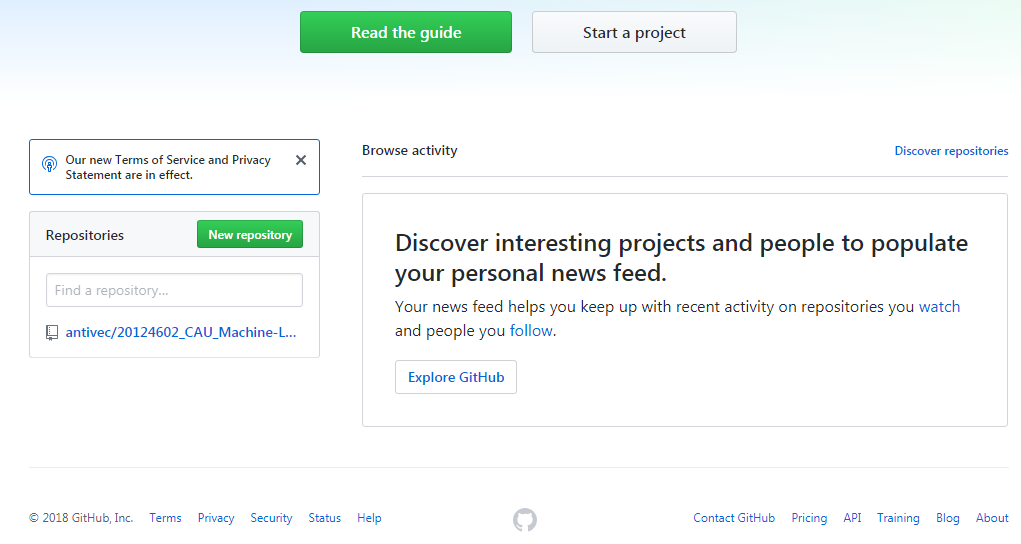
\includegraphics[width=0.75\textwidth]{main_github}
   	\caption{개인github 메인화면}
   \end{figure}
	\subsection{프로젝트 시작하기}
  	github에 개인용 또는 팀용 프로젝트를 시작하려면 다음과 같은 간단한 과정 걸쳐야 한다.
  	\begin{mdframed}[
  		linecolor= black,
  		roundcorner=10pt,
  		innertopmargin =\topskip,
  		leftmargin = 0.5cm,
  		rightmargin = 0.5cm,
  		frametitleaboveskip = 0.5pt,
  		frametitlerulewidth = 0.5pt,
  		frametitlealignment =,
  		frametitlebackgroundcolor = yellow,			
  		frametitle = {githhub 가입하기}	]
  		\begin{enumerate}
  			\item Start a Project 클릭
  			
  			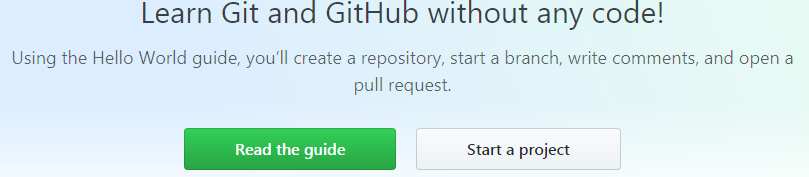
\includegraphics[width=0.75\textwidth]{start}
  			\item Repository name에 프로젝트의 이름 및 설명 입력
  			
  			 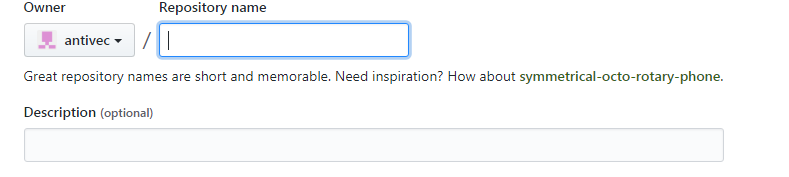
\includegraphics[width=0.75\textwidth]{owner}
  			\item 프로젝트의 공개여부와 README.md 파일 생성 유무를 설정  			
  			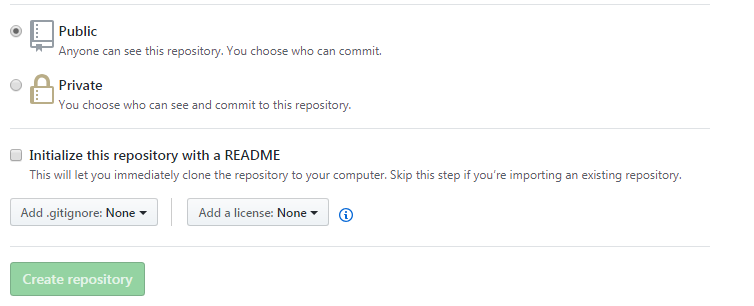
\includegraphics[width=0.75\textwidth]{publc}
  		\end{enumerate}  		
  	\end{mdframed} 
  최종적으로 다음과 같은 프로젝트가 공간이 생길것이다.  
  \begin{figure}[!hbp] 
  	\label{create_repository}
  	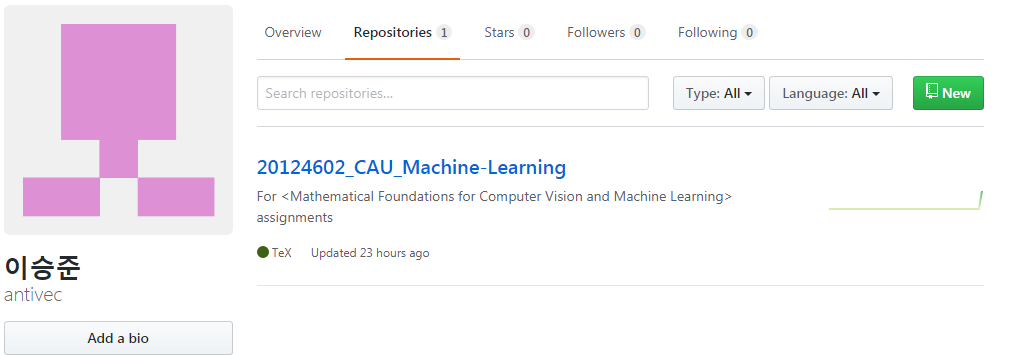
\includegraphics[width=0.65\textwidth]{create_repository}
  	\caption{\textsl{repository 생성후}}
  \end{figure}

\section{git 활용하기}
	\textit{\href{https://git-scm.com/download/win}{git홈페이지}}에 들어가 git을 설치하게 되면 다음과 같은(figure3) cmd창을 실행할 수 있다
	\begin{figure}		
		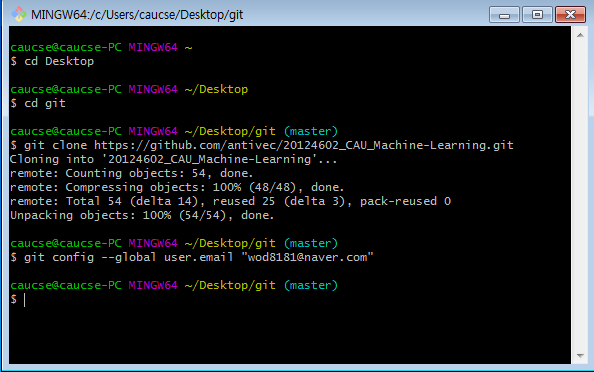
\includegraphics[width=0.75\textwidth]{git_cmd}
		\caption{개인github 메인화면}
	\end{figure}

	
	기본적인 명령어는 windows cmd와 많이 흡사하다.
	이를 통해 OS환경에 구속되지 않고 프로젝트를 업로드하거나 다운로드 받는것이 가능하다.
	
	우선적으로 git에서 프로젝트를 다운받거나 업로드를 하기 위해선 해당 폴더에 git환경을 조성해야한다.명령어는 다음과 같다.
	\begin{mdframed}[
		linecolor= black,
		roundcorner=10pt,
		innertopmargin =\topskip,
		leftmargin = 0.5cm,
		rightmargin = 0.5cm,
		frametitleaboveskip = 0.5pt,
		frametitlerulewidth = 0.5pt,
		frametitlealignment =,
		frametitlebackgroundcolor = yellow,			
		frametitle = {git환경 설정하기}	]
		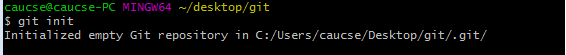
\includegraphics[width=\textwidth]{git_init}
		git init		
	\end{mdframed}
	해당 폴더의 git환경이 설정이 완료가 되면 해당 폴더의 사용자의 프로필을 설정하여야 한다
	\begin{mdframed}[
		linecolor= black,
		roundcorner=10pt,
		innertopmargin =\topskip,
		leftmargin = 0.5cm,
		rightmargin = 0.5cm,
		frametitleaboveskip = 0.5pt,
		frametitlerulewidth = 0.5pt,
		frametitlealignment =,
		frametitlebackgroundcolor = yellow,			
		frametitle = {git프로필 설정하기}	]
		\begin{enumerate}
			\item git config --global user.name = ""		
			\item git config --global user.email = ""	

		\end{enumerate}  		
	\end{mdframed}
	\subsection{github로부터 프로젝트 받기}
	앞선 그림처럼 git환경 초기화가 성공했을경우, githhub에 올린 프로젝트를 다음과 같은 명령어로 해당 폴더에 다운받을수 있다
		\begin{mdframed}[
			linecolor= black,
			roundcorner=10pt,
			innertopmargin =\topskip,
			leftmargin = 0.5cm,
			rightmargin = 0.5cm,
			frametitleaboveskip = 0.5pt,
			frametitlerulewidth = 0.5pt,
			frametitlealignment =,
			frametitlebackgroundcolor = yellow,			
			frametitle = {git환경 설정하기}	]
			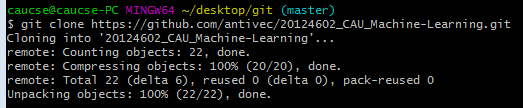
\includegraphics[width=\textwidth]{git_clone}
			- git clone  \href{https://github.com/antivec/20124602_CAU_Machine-Learning}{다운받고자 하는 github의 주소} .git	
		\end{mdframed}
		
		
  %	\href{https://github.com/antivec/20124602_CAU_Machine-Learning}{github 주소}
  % This is a comment; it will not be shown in the final output.
  % The following shows a little of the typesetting power of LaTeX:


\end{document}

  $ pdflatex assignment01.tex